\documentclass[a4paper,11pt,exos]{nsi} % COMPILE WITH DRAFT


%\pagestyle{empty}
\begin{document}

\setlength{\columnseprule}{0pt}
\setlength{\columnsep}{1cm}

\classe{\premiere spe}
\titre{Fonctions dérivées et applications}
\maketitle

\subsection*{Calculs de dérivées}
\exo{ Dérivée d'une somme}
Soit $f$ une fonction définie sur un ensemble $I$.\\
Dans chaque cas, préciser son ensemble de dérivabilité $D_{f'}$ et déterminer sa dérivée $f'$.
\begin{enumerate}
	\item 	$f(x)=2022 \quad$ et $\quad I=\R\quad$\dotfill
	\item 	$f(x)=4x+7 \quad$ et $\quad I=\R\quad$\dotfill
	\item	$f(x)=x^4 \quad$ et $\quad I=\R\quad$\dotfill
	\item	$f(x)=4x^4 \quad$ et $\quad I=\R\quad$\dotfill
	\item	$f(x)=x^3+x^2 \quad$ et $\quad I=\R\quad$\dotfill
	\item	$f(x)=x^3-x^2-x-1 \quad$ et $\quad I=\R\quad$\dotfill
	\item	$f(x)=\sqrt{x}+x \quad$ et $\quad I=\fio{0}{+\infty}\quad$\dotfill
	\item	$f(x)=x^2-\dfrac{1}{x} \quad$ et $\quad I=\R^*\quad$\dotfill
\end{enumerate}



\exo{ Dérivée d'un produit}
Soit $f$ une fonction. Dans chaque cas, préciser son ensemble de définition $D_f$, son ensemble de dérivabilité $D_{f'}$ et déterminer sa dérivée $f'$.
\begin{multicols}{2}
	\begin{enumerate}
		\item 	$f(x)=(2x-1)(x+3)$.
		\item	$f(x)=(2x+3)(1-4x)$.
		\item 	$f(x)=(x^2-x+2)(2x^3-4)$.
		\item	$f(x)=(x^2-1)(x^3+x)$.
		\item	$f(x)=\sqrt{x}(x+1)$.
		\item	$f(x)=\sqrt{x}(x^2-x+1)$.
		\item	$f(x)=\dfrac{1}{x}(x^2-1)$.
		\item	$f(x)=x^2\left(\sqrt{x}+1\right)$.
	\end{enumerate}
\end{multicols}


\exo{ Dérivée d'un inverse}
Soit $f$ une fonction. Dans chaque cas, préciser son ensemble de définition $D_f$, son ensemble de dérivabilité $D_{f'}$ et déterminer sa dérivée $f'$.
\begin{multicols}{3}
	\begin{enumerate}
		\item 	$f(x)=\dfrac{1}{x+2}$.
		\item 	$f(x)=\dfrac{1}{x^2+1}$.	
		\item	$f(x)=\dfrac{1}{\sqrt{x}}$.
		\item	$f(x)=\dfrac{1}{x^2+x+1}$.
		\item	$f(x)=\dfrac{-2}{x^2+x+1}$.
		\item	$f(x)=\dfrac{3}{x^4+1}$.
	\end{enumerate}
\end{multicols}


\exo{ Dérivée d'un quotient}
Soit $f$ une fonction définie sur un ensemble $I$. Dans chaque cas, préciser son ensemble de dérivabilité $D_{f'}$ et déterminer sa dérivée $f'$.
\begin{multicols}{2}
	\begin{enumerate}
		\item 	$f(x)=\dfrac{x+1}{x-2}\ ; \quad I=\R \backslash\left\{2\right\}$.
		\item 	$f(x)=\dfrac{x^3+1}{x^2-1}\ ; \quad I=\R \backslash\left\{-1;1\right\}$.
		\item	$f(x)=\dfrac{\sqrt{x}}{x-1}\ ; \quad I=\oio{1}{+\infty}$.
		\item	$f(x)=\dfrac{x^2+x+1}{\sqrt{x}}\ ; \quad I=\oio{0}{+\infty}$.
	\end{enumerate}
\end{multicols}
\vspace{0.5cm}


\exo{ Dérivée de $g:x\mapsto f(ax+b)$}\
Soit $f$ une fonction définie sur un ensemble $I$. Dans chaque cas, préciser son ensemble de dérivabilité $D_{f'}$ et déterminer sa dérivée $f'$.
\begin{multicols}{2}
	\begin{enumerate}
		\item 	$f(x)=(3x+1)^3\ ; \quad I=\R$.
		\item 	$f(x)=(1-2x)^4\ ; \quad I=\R$.
		\item	$f(x)=\sqrt{2x+1}\ ; \quad I=\fio{-\dfrac{1}{2}}{+\infty}$.
		\item	$f(x)=\sqrt{2-3x}\ ; \quad I=\oif{-\infty}{\dfrac{2}{3}}$.	
	\end{enumerate}
\end{multicols}



\exo{}
Soit la fonction $f$ définie sur $\R$ par $f(x)=\dfrac{2x}{x^2+1}$ dont on donne la courbe représentative $\mathcal{C}_f$ dans un repère orthonormé $\rep$.\\

\begin{minipage}{9cm}
		\begin{enumerate}
		\item 	Déterminer $D_{f'}$ l'ensemble de dérivabilité de $f$ et calculer $f'(x)$ pour $x\in D_{f'}$.
		\item 	$\mathcal{C}_f$ admet-elle une tangente parallèle à l'axe des abscisses ? Si oui, préciser en quel(s) point(s).
		\item	Déterminer une équation de chaque tangente obtenue à la question \textbf{2}.	
	\end{enumerate}
\end{minipage}
\begin{minipage}{8cm}
	\begin{center}
		\begin{tikzpicture}[scale=1.2]
			\draw[fill=white] (-3,-2) rectangle (3,2);
			\reperev{-3}{-2}{3}{2}
			\clip (-3,-2) rectangle (3,2);
			\def\F{(2*\x)/(\x*\x+1)}
			\draw [thick, domain = -3:3, samples = 100] plot( \x,{\F});
			
			\draw (-2.5,-1)node{$\courbe{f}$};
			
		\end{tikzpicture}
	\end{center}
\end{minipage}

%\subsubsection*{Applications de la dérivation}

\subsection*{Dérivée et sens de variation}

\begin{minipage}{10cm}
	\exo{}
	La courbe ci-contre représente une fonction $f$ définie et dérivable sur l'intervalle $\fif{-2}{5}$.
	\begin{enumerate}
		\item 	Par lecture graphique, déterminer le sens de variation de $f$ sur $\fif{-2}{5}$.
		\item 	Donner, suivant les valeurs de $x$, le signe de $f'(x)$ sur l'intervalle $\fif{-2}{5}$.
	\end{enumerate}
\end{minipage}
\begin{minipage}{7cm}
	\begin{flushright}
		\includegraphics[width=6cm]{courbe1}
	\end{flushright}
\end{minipage}


\begin{minipage}{6cm}
	\includegraphics[width=5cm]{courbe2}
\end{minipage}
\begin{minipage}{11cm}
	\exo{}
	La courbe ci-contre représente une fonction $g$ définie et dérivable sur l'intervalle $\fif{-4}{2}$.
	\begin{enumerate}
		\item 	Par lecture graphique, déterminer le sens de variation de $g$ sur $\fif{-4}{2}$.
		\item 	Donner, suivant les valeurs de $x$, le signe de $g'(x)$ sur l'intervalle $\fif{-4}{2}$.
	\end{enumerate}
\end{minipage}


\exo{}
$f$ est une fonction définie et dérivable sur l'intervalle $I=\fif{2}{8}$. Le tableau ci-dessous donne le signe de $f'(x)$ sur $I$.
\begin{center}
	\begin{tikzpicture}
		\tkzTabInit[color,lgt=3.5,espcl=3]
		{$x$ /.7 ,$f'(x)$ /.7}
		{2, 3 ,5, 8 }
		\tkzTabLine{,+ , z, +,z,-,}
	\end{tikzpicture}
\end{center}
Dresser le tableau de variations de $f$ sur $I$.


\exo{}
$g$ est une fonction définie et dérivable sur l'intervalle $I=\fio{0}{+\infty}$. Le tableau ci-dessous donne le signe de $g'(x)$ sur $I$.
\begin{center}
	\begin{tikzpicture}
		\tkzTabInit[color,lgt=3.5,espcl=3]
		{$x$ /.7 ,$g'(x)$ /.7}
		{0, 3 , 6 , $+\infty$ }
		\tkzTabLine{,- , z, +,z,-,}
	\end{tikzpicture}
\end{center}
\begin{enumerate}
	\item 	Sachant que $g(3)=-1$ et $g(6)=2$, dresser le tableau de variations de $g$.
	\item 	Tracer une courbe susceptible de représenter la fonction $g$.	
\end{enumerate}

\begin{minipage}{8cm}
	\exo{}
	On considère la fonction $f$ dont la représentation graphique dans un repère orthonormé est donnée ci-contre.\\

	Parmi les trois courbes suivantes, quelle est la seule susceptible de représenter la fonction dérivée de $f$ ?
\end{minipage}
\begin{minipage}{9cm}
	\begin{flushright}
		\includegraphics[width=8cm]{courbe3}
	\end{flushright}
\end{minipage}
\begin{center}
	\includegraphics[width=10cm]{courbe4}
\end{center}


\exo{}
$f$ est la fonction définie par $f(x)=-x^3+x^2-x$. $f'$ est la fonction dérivée de $f$.
\begin{enumerate}
	\item 	Préciser $\mathcal{D}_f$, ensemble de définition et de dérivabilité de $f$.
	\item 	Calculer $f'(x)$ puis vérifier que , pour tout $x\in \mathcal{D}_f, f'(x)=-2x^2-(x-1)^2$.
	\item	\'Etudier le signe de $f'(x)$ puis dresser le tableau de variations de $f$ sur $\mathcal{D}_f$.	
\end{enumerate}


\exo{}
$g$ est la fonction définie par $g(x)=\dfrac{x^2+3}{x+1}$.
\begin{enumerate}
	\item 	Préciser l'ensemble de définition de $g$.
	\item 	Calculer $g'(x)$ puis vérifier que $g'(x)=\dfrac{(x-1)(x+3)}{(x+1)^2}$.
	\item	\'Etudier le signe de $g'(x)$ puis dresser le tableau de variations de $f$ sur son ensemble de définition.	
\end{enumerate}


\exo{}
$h$ est la fonction définie sur $\oio{0}{+\infty}$ par $h(x)=\dfrac{x+1}{\sqrt{x}}$. $h'$ est la fonction dérivée de $h$.
\begin{enumerate}
	\item 	Justifier la dérivabilité de $h$ sur $\oio{0}{+\infty}$.
	\item 	Vérifier que $h'(x)=\dfrac{x-1}{2x\sqrt{x}}$.
	\item	En déduire les variations de $h$ sur $\oio{0}{+\infty}$.
\end{enumerate}



\subsection*{Extremums d'une fonction}
\exo{}
La courbe ci-dessous représente une fonction $h$ définie sur $\fif{-8}{6}$.\\
\begin{minipage}{9cm}
	\begin{enumerate}
		\item 	Quel est le maximum local de $h$ sur $\fif{-8}{-4}$ ?
		\item 	Quel est le minimum local de $h$ sur $\fif{-8}{0}$ ?
		\item	Quel est le maximum de $h$ sur $\fif{-8}{6}$ ?
		\item	Quel est le minimum de $h$ au voisinage de 3 ?	
	\end{enumerate}
\end{minipage}
\begin{minipage}{8cm}
	\begin{flushright}
		\includegraphics[width=8cm]{courbe5}
	\end{flushright}
\end{minipage}


\exo{}
Dans chaque cas :
\begin{enumalph}
	\item 	Construire le tableau de variations de $f$ sur son ensemble de définition.
	\item 	Donner, suivants les valeurs de $x$, le signe de $f(x)$.	
\end{enumalph}
\begin{multicols}{2}
	\begin{enumerate}
		\item 	$f$ est une fonction définie et dérivable sur $\R$ telle que, pour tout $x\in \R, f'(x)>0$ et $f(-2)=0$.
		\item 	$f$ est une fonction définie et dérivable sur $\R$ telle que, pour tout $x\in \oio{-\infty}{2}, f'(x)>0$ et, pour tout $x\in\oio{2}{+\infty}, f'(x)<0$.\\
		On sait de plus que $f'(2)=0$ et $f(2)=-1$.
	\end{enumerate}
\end{multicols}

\exo{}
On donne ci-dessous le tableau de variations d'une fonction $f$ définie sur $\mathcal{D}=\fio{-3}{0}\cup\oif{0}{5}$.
\begin{center}
	\includegraphics[width=8cm]{tableau1}
\end{center}
\begin{enumerate}
	\item 	\'Ecrire une équation pour chacune des tangentes à la courbe représentative de $f$ que le tableau de variations permet de connaître.
	\item 	Tracer une courbe compatible avec le tableau de variations.	
	\begin{center}
		\includegraphics[width=10cm]{courbe6}
	\end{center}
\end{enumerate}



\exo{ QCM}
\begin{enumerate}
	\item 	On donne ci-dessous la courbe $C_f$, représentative d'une fonction $f$ définie sur $\fif{-5}{3}$. $f'$ est la fonction dérivée de $f$.
    \begin{center}
        \includegraphics[width=8cm]{qcm}
    \end{center}
    \begin{qcm}
        \item $f'(0)=0$
        \item $f'(-4)<0$
        \item Pour tout $x$ de l'intervalle $\fif{-3}{1}, f'(x)\leqslant0$.
        \item $f'$ s'annule une seule fois sur $\fif{-5}{3}$.
    \end{qcm}
   
	\item 	$f$ est la fonction définie sur $\R$ par $f(x)=x^3-4,8x-3$.
	\begin{qcm}
        \item $f$ est strictement croissante sur $\R$.
        \item $f$ admet un seul extremum local sur $\R$.
        \item 3,2 est un minimum local de $f$ sur $\R$.
        \item $f$ admet deux extremums locaux sur $\R$.
    \end{qcm}
    
	\item	$g$ est la fonction définie sur $\fio{0}{+\infty}$ par $g(x)=x-4\sqrt{x}$.
	\begin{qcm}
        \item Pour tout $x$ de l'intervalle $\fio{0}{+\infty}, g(x)\geqslant 0$.
        \item $g(4)$ est le maximum de $g$ sur $\fio{0}{+\infty}$.
        \item $g'(4)=g(4)=0$.
        \item $g$ est croissante sur $\fio{4}{+\infty}$.
    \end{qcm}
    
	\item	$g$ est la fonction définie sur $\oio{-\infty}{2}\cup\oio{2}{+\infty}$ par $g(x)=\dfrac{4-5x}{x-2}$.
	\begin{qcm}
        \item $g$ est strictement croissante sur $\R$.
        \item $g$ est strictement croissante sur $\oio{-\infty}{2}\cup\oio{2}{+\infty}$.
        \item $g$ est strictement croissante sur $\oio{-\infty}{2}$.
        \item 6 est le maximum de $g$ sur $\oio{-\infty}{2}$.
    \end{qcm}
\end{enumerate}


\exo{}
$h$ est la fonction définie sur $\fio{0}{+\infty}$ par $h(x)=\sqrt{x}\left(x^2-1\right)$. $h'$ est la fonction dérivée de $h$.
\begin{enumerate}
	\item 	Justifier la dérivabilité de $h$ sur $\oio{0}{+\infty}$.
	\item 	Vérifier que $h'(x)=\dfrac{\left(x\sqrt{5}+1\right)\left(x\sqrt{5}-1\right)}{2\sqrt{x}}$.
	\item	\'Etudier le signe de $h'(x)$ puis dresser le tableau de variations de $h$ sur $\fio{0}{+\infty}$.
	\item	Déterminer l'extremum de $h$ sur $\fio{0}{+\infty}$.
\end{enumerate}


\exo{}
Soit $h$ la fonction définie sur $\R$ par $h(x)=-9x^4+x^3$.\\
Maël a représenté cette fonction à la calculatrice pour dresser son tableau de variations.

\begin{minipage}{9.5cm}
	\begin{enumerate}
		\item 	À partir de cette représentation, comment dresser le tableau de variations de $h$ ? $h$ admet-elle un maximum ?
		\item 	On note $h'$ la fonction dérivée de $h$ sur $\R$.
		\begin{enumalph}
			\item 	Déterminer l'expression de $h'$.
			\item 	En déduire le tableau de variations de $h$ sur $\R$ ainsi que le maximum de $h$.	
		\end{enumalph}	
	\item	Proposer à Maël une fenêtre d'affichage permettant de voir les résultats obtenus à la question \textbf{2}.
	\end{enumerate}
\end{minipage}
\begin{minipage}{7.5cm}
	\begin{flushright}
		\includegraphics[width=7cm]{calculatrice}
	\end{flushright}
\end{minipage}


\exo{}
On donne ci-dessous le tableau de variations d'une fonction $f$ définie et dérivable sur $\mathcal{D}=\fio{-3}{0}\cup\oif{0}{5}$.
\begin{center}
	\includegraphics[width=10cm]{tableau2}
\end{center}
Pour chacune des affirmations ci-dessous, indiquer si elle est vraie ou fausse en justifiant la réponse.
\begin{enumerate}
	\item 	Pour tout $x\in\oif{0}{5}, f(x)>0$.
	\item 	$f$ est strictement croissante sur $\fio{-3}{0}\cup\oif{0}{1}$.
	\item	Si $f(x)\in \fif{1}{3}$ alors $x\in\fif{1}{4}$.
	\item	$T$ est la tangente à la courbe représentative de $f$ au point d'abscisse 1. Une équations de $T$ est : $2x-y-1=0$.	
\end{enumerate}

\subsubsection*{Exercices de synthèse}
\exo{ Coût marginal}
Une entreprise fabrique des articles de luxe dont le coût mensuel de production pour une quantité de $q$ dizaines d'objets s'exprime, en euro, par la fonction définie par :
\begin{center}
	$C(q)=15q^3-120q^2+350q+1000\quad$ avec $\quad q>0$.
\end{center}
On appelle \textbf{coût marginal de production} la variation du coût total de production pour un article supplémentaire. Quand la quantité d'articles $q$ est très importante, on admet que le coût marginal peut être approché par la dérivée $C'(q)$.
\begin{enumerate}
	\item 	Calculer le coût marginal $\quad C_m(q)=C(q+1)-C(q)$.
	\item 	Calculer $C'(q)$.
	\item	On étudie l'erreur commise en assimilant le coût marginal $C_m(q)$ à la dérivée $C'(q)$.
	\begin{enumalph}
		\item 	 Calculer $E(q)=C'(q)-C_m(q)$.
		\item 	 Déterminer le nombre minimal d'objets à fabriquer pour que l'erreur commise soit inférieure à 1 \%.
	\end{enumalph}
\end{enumerate}	



\exo{}
\begin{minipage}{8cm}
	Une entreprise fabrique des rétroviseurs pour voitures. la fonction « coût total » est définie sur $I=\fif{0}{11}$ par :
	 $$C(x)=0,3x^3-3x^2+9x+6$$
	$C(x)$ est exprimée en milliers d'euros et $x$ est le nombre de milliers d'articles fabriqués. Le prix de vente de 1000 articles est 8025 €. On suppose que chaque article fabriqué est vendu.\\
	La courbe représentative de la fonction $C$ est représentée ci-contre dans un repère orthogonal.
\end{minipage}
\begin{minipage}{9cm}
	\begin{center}
		\includegraphics[width=8cm]{retroviseurs}
	\end{center}
\end{minipage}

\begin{enumerate}
	\item 	On note $R$ la fonction recette, exprimée en milliers d'euros, relative à la vente de $x$ milliers d'articles.
	\begin{enumalph}
		\item 	Expliquer pourquoi $R(x)=8,025x$.
		\item 	Tracer la courbe représentative de $R$ dans le repère ci-dessus.
		\item	Déterminer graphiquement l'intervalle de production qui permet de réaliser un bénéfice.
		\item	Déterminer graphiquement la quantité $x_0$ que l'entreprise doit fabriquer pour réaliser un bénéfice maximal.	
	\end{enumalph}
	\item 	Le bénéfice réalisé par cette entreprise est donné, en milliers d'euros, par la fonction $B$ définie et dérivable sur $I$. On note $B'$ la fonction dérivée de $B$.
	\begin{enumalph}
		\item 	Montrer que, pour tout $x\in I, B'(x)=-0,075(6x-1)(2x-13)$.
		\item 	\'Etudier le signe de $B'(x)$ puis dresser le tableau de variations de $B$.
		\item	Retrouver, à partir du tableau de variations, la valeur de $x_0$. Justifier.
		\item	Quel est le montant, en euros, du bénéfice maximal ?	
	\end{enumalph}	
\end{enumerate}


\exo{}
\begin{minipage}{10cm}
	$[AC]$ est un segment de longueur 12 cm. $B$ est un point du segment $[AC]$ tel que $AB=x$. On construit d'un même côté de la droite $(AB)$ les demi-cercles de diamètres $[AB], [BC]$ et $[AC]$.\\
	On note $S(x)$ l'aire de la surface hachurée en fonction de $x$.
\end{minipage}
\begin{minipage}{7cm}
	\begin{center}
		\includegraphics[width=6cm]{aire}
	\end{center}
\end{minipage}
\begin{enumerate}
	\item 	Quel est l'ensemble de définition $\mathcal{D}_S$ de la fonction $S$ ?
	\item 	Montrer que, pour tout $x\in \mathcal{D}_S,\quad S(x)=\dfrac{\pi}{4}\left(12x-x^2\right)$.
	\item	Déterminer la valeur $x_0$ pour laquelle l'aire de la partie hachurée est maximale.
\end{enumerate}



%\begin{minipage}{11cm}
	\exo{}
	Mélissa souhaite construire un cerf-volant d'aire maximale. Pour le confectionner, elle possède un bâton de longueur 180 cm qu'elle devra couper en deux.\\
	On rappelle que les diagonales $(AC)$ et $(BD)$ sont perpendiculaires et que l'aire d'un tel cerf-volant est égale à $\dfrac{AC\times BD}{2}$.
%\end{minipage}
%\begin{minipage}{6cm}
	\begin{center}
		\begin{tikzpicture}[scale=.3]
			%\draw [thin,UGLiBlue] (-0,0) grid (10,10);	
			\coordinate (B) at (0,0);
			\coordinate (D) at (15,0);
			\coordinate (C) at (5,4);
			\coordinate (A) at (5,-4);
			\fill[UGLiOrange] (A) -- (B) -- (C) -- (D)-- cycle ;
			\draw[thick] (A) node[below]{A} -- (C) node[above]{C} ;
			\draw[thick] (B) node [left]{B} -- (D) node[right]{D} ;
		\end{tikzpicture}
	\end{center}
%\end{minipage}
Déterminer la longueur des diagonales pour satisfaire Mélissa. Préciser alors l'aire de son cerf-volant.

\exo{}
\begin{minipage}{12cm}
	Le circuit électrique schématisé ci-contre comprend :
	\begin{enumerate}[label=\textbullet]
		\item 	un générateur de f.é.m (force électromotrice) fixe $U_0=12$ volts ;
		\item 	une résistance fixe $R_0=6$ ohms;
		\item	une résistance variable $R$ en ohms.	
	\end{enumerate}
\end{minipage}
\begin{minipage}{5cm}
	\includegraphics[width=5cm]{circuit}\\[1em]
\end{minipage}
On admet que le puissance (en watt) dissipée dans la résistance $R$, en fonction de $U_0$ et de $R_0$, est donnée par la fonction $P$ définie sur $K=\fio{0}{+\infty}$ par $P(R)=\dfrac{U_0 ^2R}{\left(R+R_0\right)^2}$.
\begin{enumerate}
	\item 	Avec les valeurs données dans l'énoncé, écrire l'expression de la fonction $P$ et déterminer sa dérivée.
	\item 	\'Etudier les variations de la fonction $P$ sur $K$.
	\item	Déterminer la valeur à donner à la résistance $R$ pour que la puissance dissipée soit maximale.
	\item	\begin{enumalph}
		\item 	À la calculatrice, tracer la représentation graphique de la fonction $P$.
		\item 	Àl'aide du graphique, conjecturer pour quelles valeurs de $R$ la puissance est supérieure à 4,5 watts.
		\item	Vérifier, par le calcul, les résultats précédents.	
	\end{enumalph}
\end{enumerate}


\exo{}
On définit la fonction $f$ sur $\R$ par $f(x)=x^3+ax^2+ax$ où $a$ est un réel fixé.\\
Pour quelles valeurs de $a$ la fonction $f$ est-elle strictement croissante sur $\R$ ?\\


\exo{}
\begin{multicols}{2}
	$f$ est une fonction polynôme du troisième degré définie sur $\R$ par $f(x)=ax^3+bx^2+cx+d$ où $a,b,c$ et $d$ sont des réels donnés avec $a\neq 0$. $f'$ est la fonction dérivée de $f$.
	\begin{enumerate}
		\item 	Exprimer $f'(x)$ en fonction de $a,b,c$ et $x$.
		\item 	Démontrer que $f$ admet deux extremums locaux sur $\R$ si, et seulement si, $4b^2-12ac>0$.
		\item	Compléter le script suivant:
	\end{enumerate}	
\begin{pyc}
    \begin{minted}{python}
D = 4*b**2-12*a*c
if D>0 :
    print(...................)
elif a>0 :
    print(...................)
else :
    print(...................)        
    \end{minted}
\end{pyc}


\end{multicols}


\end{document}
